\chapter{Metodolog\'ia.}

\section{Elaboraci\'on de la base de datos.}


\hspace{0.4cm} La fuente principal de informaci\'on para calcular la curva de rendimientos para los t\'itulos de la deuda p\'ublica nacional es el Banco Central de Venezuela (BCV), el cual diariamente publica las operaciones realizadas con estos instrumentos y los publica en el documento ``resumersec"\hspace{0.01cm}  (Ver Figura \ref{doc_bcv}). Es importante destacar, que en este documento se encuentran por d\'ia dos pesta\~nas, la $``0-22"$ y la $``0-23"$, en la primera pesta\~na se encuentran las operaciones interbancarias, por su parte la segunda pesta\~na muestra informaci\'on sobre las operaciones realizadas por entes privados, en este caso el precio pautado en la operaci\'on no est\'a disponible, raz\'on por la cual esta pesta\~na no se toma en consideraci\'on. La informaci\'on disponible en la pesta\~na $``0-22"$ es la siguiente,

\begin{itemize}
  \item C\'odigo del instrumento: c\'odigo \'unico que se asocia a cada instrumento.
  \item Fecha de vencimiento: fecha de maduraci\'on de cada instrumento.
  \item Plazo: cantidad de d\'ias que faltan para que el instrumento venza.
  \item Cantidad de operaciones: n\'umero de operaciones realizadas con cada instrumento.
  \item Monto en Bol\'ivares: monto total involucrado en la operaci\'on.
  \item Precio m\'inimo: precio m\'as bajo pautado en la operaci\'on.
  \item Precio m\'aximo: precio m\'as alto pautado en la operaci\'on.
  \item Precio promedio: precio promedio pautado en la la operaci\'on. Cabe destacar que si existe una s\'ola operaci\'on, los precios m\'inimo, m\'aximo y promedio ser\'an iguales.
  \item Cup\'on: tasa de inter\'es pagadera por cada instrumento.
\end{itemize}


\vspace{0.5cm}

\begin{figure}[h]
  \scalebox{0.50}{\includegraphics{images/Imagen022.png}}
%\includegraphics[width=0.7\textwidth]{Imagen022.png}
\caption{Pesta\~na ``0-22".}
\label{doc_bcv}
\end{figure}

\vspace{0.5cm}

\hspace{0.4cm} Es importante recordar que dentro de los t\'itulos de la deuda p\'ublica nacional se encuentran los t\'itulos de inter\'es fijo (TIF) y los t\'itulos de tasa variable (VEBONO), los primeros se caracterizan por poseer una tasa de cup\'on que no varia, por su parte los VEBONO poseen una tasa de inter\'es variable.

\vspace{0.5cm}

\hspace{0.4cm}Esta informaci\'on tambi\'en es suministrada por el BCV, en su documento de las ``Caracter\'isticas de la deuda p\'ublica nacional" (Ver Figura \ref{doc_carac}), por lo cual el mismo se debe revisar con cierta frecuencia, con el fin de actualizar la tasa de cup\'on de los VEBONO. En este documento se muestra informaci\'on que caracteriza a cada instrumento, el mismo posee varias pesta\~nas, en este trabajo s\'olo se considerar\'a la pesta\~na $``DPN"$ en donde se encuentra informaci\'on sobre los instrumentos emitidos en moneda nacional. La informaci\'on disponible en este documento se muestra a continuaci\'on,

\begin{itemize}
  \item N\'umero-emisi\'on-decreto: informaci\'on sobre emisi\'on de cada instrumento.
  \item C\'odigo: c\'odigo \'unico que se asocia a cada instrumento.
  \item Fecha de emisi\'on: fecha cuando se emiti\'o cada instrumento.
  \item Fecha de vencimiento: fecha de maduraci\'on de cada instrumento.
  \item Monto en circulaci\'on: monto total de cada instrumento en circulaci\'on.
  \item Porcentaje de referecia: indica si el instrumento es de tasa fija o tasa variable.
  \item Fecha de inicio: indica cada cuanto tiempo el instrumento paga cup\'on.
  \item Per\'iodo vigente: indica el per\'iodo (fecha inicio y fecha fin) cuando cada instrumento paga cup\'on.
  \item Tasa: cup\'on asociado a cada instrumento.
\end{itemize}



\begin{figure}[h]
  \scalebox{0.50}{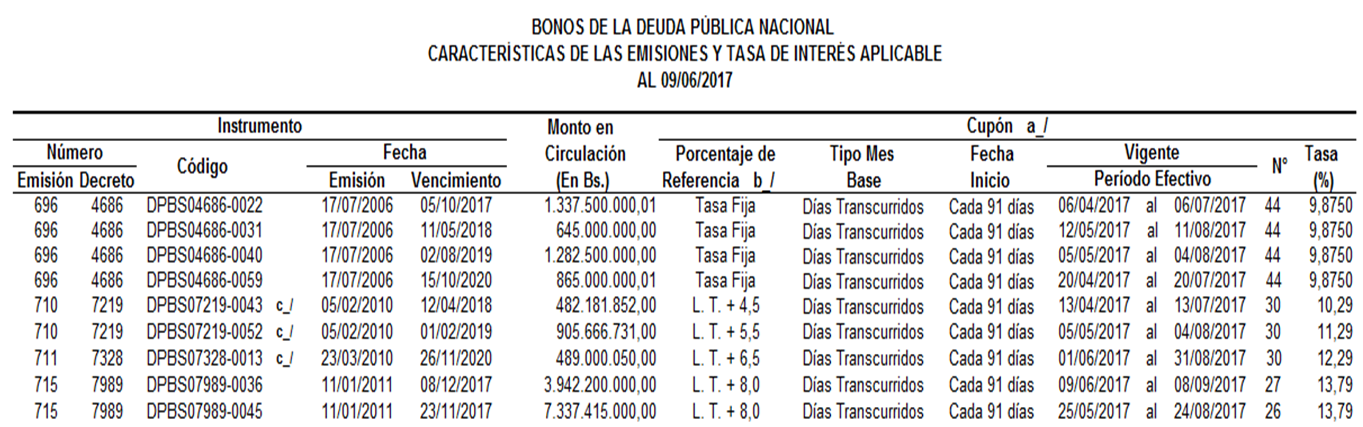
\includegraphics{images/Imagencarac.png}}
\caption{Caracter\'isticas.}
\label{doc_carac}
\end{figure}


\hspace{0.4cm} A partir de la pesta\~na ``0-22"\hspace{0.01cm} y del documento de las caracter\'isticas, se cre\'o la base de datos con la cual se va a trabajar, la misma contiene no s\'olo la informaci\'on suministrada por la pesta\~na ``0-22", sino alguna informaci\'on adicional tomada del documento de las caracter\'isticas. En dicha base de datos se contar\'a con la siguiente informaci\'on,

\vspace{0.5cm}

\begin{itemize}
  \item Tipo instrumento: indica el tipo de instrumento.
  \item Nombre: proporciona el nombre corto del t\'itulo, usualmente este nombre se conforma por el tipo de t\'itulo m\'as su mes y a\~no de vencimiento, por ejemplo, el t\'itulo TIF032028, representa al t\'itulo TIF con vencimiento en marzo del 2028.
  \item Fecha de operaci\'on: indica la fecha en que se efectu\'o dicha operaci\'on.
  \item Fuente: indica la fuente de donde se tom\'o la informaci\'on, esta se puede tomar de dos fuentes, la primera mediante la pesta\~na 0-22 (mercado secundario) y  la otra mediante el documento de las subastas (mercado primario, informaci\'on suministrada por el BCV).
  \item Sicet: proporciona el c\'odigo asociado a cada t\'itulo.
  \item Fecha de vencimiento: indica la fecha de maduraci\'on (vencimiento) del instrumento.
  \item Plazo: indica la cantidad de d\'ias que falta para que el instrumento se venza.
  \item Cantidad de operaciones: proporciona la cantidad de operaciones efectuadas con un insrumento en espec\'ifico.
  \item Monto: indica el monto en Bol\'ivares, por el cual se efectu\'o la operaci\'on u operaciones.
  \item Precio m\'inimo: indica el precio m\'inimo, por el cual se trans\'o la operaci\'on.
  \item Precio m\'aximo: indica el precio m\'aximo, por el cual se trans\'o la operaci\'on.
  \item Precio promedio: indica el precio promedio, por el cual se trans\'o la operaci\'on, cabe destacar que en dado caso de existir una sola operaci\'on el valor del precio m\'inimo, m\'aximo y promedio van a coincidir.
  \item Cup\'on: proporciona la tasa de cup\'on asociado a cada instrumento.
  \item Frecuencia: indica con que frecuencia el instrumento paga cup\'on, para los TIF y VEBONO, esta es 4, pues los mismos pagan cu\'pon trimestralmente, as\'i se obtiene este valor pues existen 4 trimestres en el a\~no.

\end{itemize}

\vspace{0.5cm}

\hspace{0.4cm} Una vez obtenida la base de datos esta seg\'un sea el caso puede ser depurada mediante ciertos criterios, el primero es que aquellas operaciones con un monto menor a los 10 milllones no se consideran. El segundo es considerar la operaci\'on mas reciente, es decir, si en la base de datos se tiene que para un mismo instrumento existen diferentes operaciones en diferentes d\'ias, s\'olo se considerar\'a la operaci\'on m\'as reciente.

%El segundo es el tipo de fuente, siempre prevalecer\'a la fuente subasta.

\hspace{0.4cm} Para efectuar la depuraci\'on, a la base de datos anterior se le a\~nadir\'an dos columnas nuevas una que indica el rendimiento al vencimiento de cada instrumento y la otra que indica la decisi\'on que se tom\'o en base a los criterios descritos anteriormente (Ver Figura \ref{base_datos}). Esta \'ultima ser\'a una variable dicot\'omica, es decir solo con dos valores (0 \'o 1), en donde ``0" me indica que no selecciono el t\'itulo y ``1" me indica que si lo tomo en cuenta para el estudio a realizar.

\begin{figure}[h]
  \scalebox{0.50}{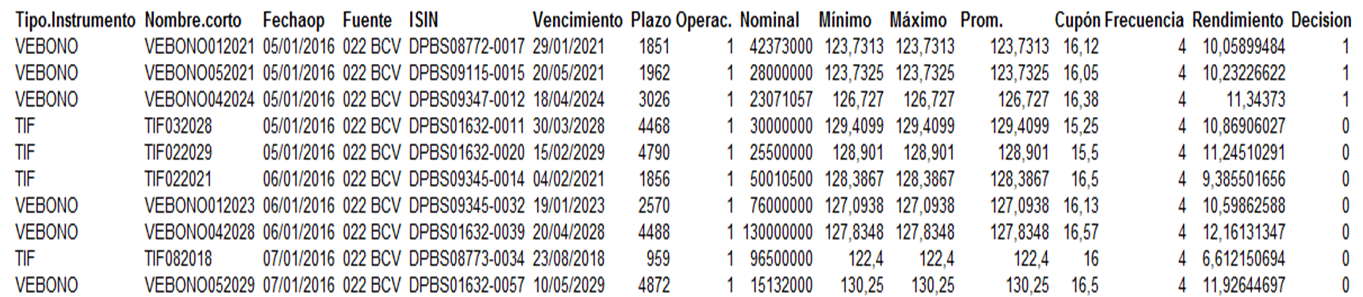
\includegraphics{images/Imagenbase.png}}
\caption{Base de datos.}
\label{base_datos}
\end{figure}


\hspace{0.4cm} Una vez calculados los precios estimados asociados a cada instrumento, se proceder\'a a comparar los mismo con aquellos obtenidos por una metodolog\'ia distinta. La metodolog\'ia con la cual se va a comparar es la de Svensson, la cual es una metodolog\'ia param\'etrica.



\hspace{0.4cm} Los instrumentos a considerar ser\'an aquellos pertencientes al portafolio de inversiones de una instituci\'on financiera, de tal manera que para un d\'ia especifico sea posible conocer cuanta es la ganancia o p\'erdida que generan estos instrumentos. y por ende saber si es viable la venta o compra de determinado instrumento.


\hspace{0.4cm} A partir de la data obtenida (Ver Figura \ref{base_datos}), se proceder\'a a a\~nadir unas columnas nuevas con el fin de clasificar las observaciones para los distintos instrumentos en diferentes per\'iodos de vencimiento. Los per\'iodos de vencimiento son,

\begin{itemize}
\item Corto plazo: se refiere al vencimiento m\'as cercano, los instrumentos que se encuentran aqu\'i son aquellos que poseen un vencimiento menor a un a\~no.
\item Mediano plazo: en esta clasificaci\'on se encuentran los instrumentos cuyo vencimiento este entre uno y diez a\~nos.
\item Largo plazo: hace referencia a aquellos instrumentos que tengan un vencimiento mayor a diez a\~nos.
\end{itemize}

\hspace{0.4cm} Luego de separar la data por tipo de instrumento, la nueva data con la que se trabajar\'a es la siguiente,

\begin{figure}[h]
  \scalebox{0.50}{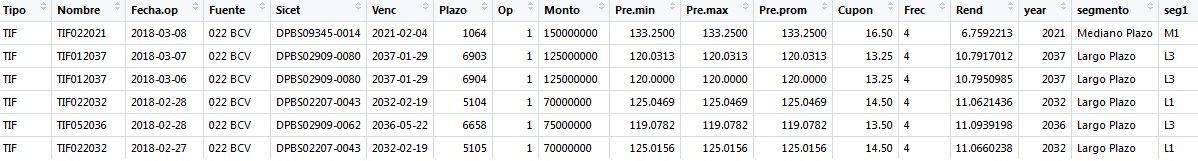
\includegraphics{images/data_nueva.png}}
\caption{Base de datos TIF.}
\label{base_datos_tif}
\end{figure}

\hspace{0.4cm} Con el fin de contar con la data m\'as reciente a partir de la fecha de valoraci\'on, se cre\'o la funci\'on ``extrae" \hspace{0.01cm} la cual selecciona de la data de la Figura (\ref{base_datos_tif}) una determinada cantidad de observaciones, la cual es especificada por el usuario, esta funci\'on cuenta con los siguientes argumentos,

\begin{itemize}
 \item fv: indica la fecha de valoraci\'on para la cual se est\'a realizando el estudio.
 \item dias: indica la cantidad de d\'ias que el usuario desea, a partir de este valor se va a obtener la data con la que se va a trabajar.
 \item data: hace referencia a la data completa para cada tipo de instrumento, a partir de la misma se procedera a extraer parte de ella a partir del n\'umero de dias seleccionado.
\end{itemize}

\hspace{0.4cm} Luego de selecionar la data, la misma se procede a depurar, es decir, se van a eliminar las observaciones duplicadas considerando s\'olo aquellas que sean m\'as recientes. 


\hspace{0.4cm}As\'i a partir de esta data s\'olo se consideraran las columnas plazo y rendimiento con el fin de tener una nube de puntos a partir de la cual se haga el ajuste de la funci\'on spline, y as\'i obtener la curva de rendimientos.

\newpage

\hspace{0.4cm} La data obtenida a partir de la depuraci\'on anterior es,

\begin{figure}[h]
    {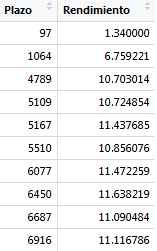
\includegraphics{images/cand.png}}
\caption{Data depurada TIF.}
\label{fig91}
\end{figure}



\hspace{0.4cm} Una vez obtenida la data para los Tif y Vebono se utiliz\'o la funci\'on ``smooth.spline" \hspace{0.01cm} del programa estad\'istico R, para ajustar un spline c\'ubico a la data ingresada. Los argumentos requeridos por esta funci\'on son los siguientes,

\begin{itemize}
  \item X: representa el vector de la variable predictiva.
  \item Y: representa el vector de la variable repuesta.
  \item cv: (TRUE/FALSE) variable del tipo l\'ogico que representa si se va a utilizar la validaci\'on cruzada generalizada al momento de calcular el par\'ametro de suavizamiento.
  \item Spar: representa el par\'ametro de suavizamiento, t\'ipicamente (aunque no necesariamente) ubicado entre 0 y 1. Es el coeficiente lambda que acompa\~na a la integral del cuadrado de la segunda derivada de la funci\'on f.
\end{itemize}

\hspace{0.4cm} De esta manera el siguiente comando ajusta un spline cubico a la data ingresada,


spline1=smooth.spline(X=datT1\$Plazo,Y=datT1\$Rendimiento,cv=TRUE, spar=1.35)


\noindent y lo guarda en la variable ``spline1".

\hspace{0.4cm} Es importante se\~nalar lo crucial de la escogencia del par\'ametro ``spar", pues de \'el depende que tan suave sea la curva, la Figura \ref{comp_spar} muestra como var\'ia la curva cuando se cambia  el valor del ``spar", para esta comparaci\'on se us\'o tres valores, el primero fue 0.51 con el cual se obtiene una curva con ciertos picos la cual no es suave en lo absoluto. 

\newpage

\hspace{0.4cm} Usando el valor de 0.71 se obtiene la curva roja la cual presenta una mayor suavidad. Mientras que usando el valor de 0.81 se obtiene un mejor resultado aunque similar al anterior. De esta manera, se puede observar la importancia de la elecci\'on correcta de este par\'ametro, mientras este valor se aproxime a 1 se obtendr\'a una curva con mayor suvidad.

\begin{figure}[h]
  {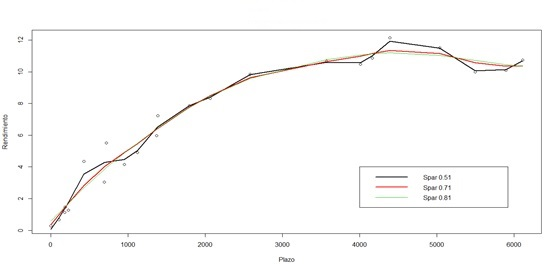
\includegraphics{images/curvavbv2.jpg}}
\caption{Curva de rendimiento Vebono para diferentes valores de suavizado.}
\label{comp_spar}
\end{figure}

\hspace{0.4cm} Cabe destacar que para cada versi\'on el par\'ametro usado en la variable ``spar" \hspace{0.2cm} cambi\'o. Esto debido a la diferente cantidad de puntos que tiene cada versi\'on. As\'i el valor del par\'ametro ``spar" \hspace{0.2cm} para los TIF se ubic\'o en el siguiente intervalo [0.4,0.6], por su parte para los VEBONOS la elecci\'on de dicho par\'ametro esta en [0.3,0.5]. Los mismos se obtuvieron mediante ensayo y error. Para los valores ubicados dentro de los intervalos mencionados siempre se obtuvo una curva suave.

\hspace{0.4cm} Una vez que se obtiene la curva estimada y es guardada en una variable (en este caso, la variable es spline1), se procede a aplicar el comando ``predict", para estimar el rendimiento de alg\'un plazo que se ingrese.

\hspace{0.4cm} As\'i con el fin de calcular el precio estimado de cada t\'itulo, se cre\'o la funci\'on ``precio"\hspace{0.01cm} mediante R, para determinar de forma autom\'atica dichos valores. Los imputs de dicha funci\'on son los siguientes,


\begin{itemize}
  \item Tit: representa el nombre de cada t\'itulo, al cual se le quiere estimar su precio, el mismo debe ser un car\'acter, ej: TIF102017 \'o VEBONO112017.
  \item Spline1: representa la variable donde se guardo la curva ajustada mediante el spline.
  \item Fv: indica la fecha de valoraci\'on, para la cual se desea conocer el precio estimado.
\end{itemize}


\hspace{0.4cm} Una vez ingresado los imputs, la funci\'on internamente busca el nombre del t\'itulo en el documento de las caracter\'isticas m\'as reciente, y extrae del mismo la fecha de pago del pr\'oximo cup\'on y su fecha de vencimiento, con el fin de crear un vector de flujos.


\hspace{0.4cm} Por ejemplo, si se quiere conocer el precio estimado del t\'itulo ``TIF032022" \hspace{0.01cm} al ``01/03/2018", la funci\'on busca su fecha de vencimiento $(03/03/2022)$ y la fecha de pago del pr\'oximo cup\'on la cual es en este caso $08/03/2018$. Luego con dichos valores calcula la Tabla \ref{tabla1}, que representa los cupones que le quedan por pagar al t\'itulo,

\renewcommand{\tablename}{Tabla}
\begin{table}[H]
\centering
%\begin{center}
{\begin{tabular}[t]{|l |c |c |c |c |c |r|}
\hline
Fecha & Plazo t\'itulo & Plazo a\~nos & Rend estimado & Exp & Cup\'on & Producto \\
\hline
08/03/2018 & 7  & 0,0191780 & 0,45\% & 0,9999131 & 4& 3,999652\\
\hline
07/06/2018 & 98 & 0,2684931 & 1,05\% & 0,9971804 & 4& 3,988721\\
\hline
06/09/2018 & 189 & 0,5178082 & 1,64\% & 0,9915025 & 4& 3,966010\\
\hline
06/12/2018 & 280 & 0,7671232 & 2,23\% & 0,9829646 & 4& 3,931859\\
\hline
07/03/2019 & 317 & 1,0164383 & 2,82\% & 0,9717013 & 4& 3,886805\\
\hline
06/06/2019 & 462 & 1,2657534 & 3,39\% & 0,9578928 & 4& 3,831571\\
\hline
05/09/2019 & 553 & 1,5150684 & 3,96\% & 0,9417596 & 4& 3,767038\\
\hline
05/12/2019 & 644 & 1,7643835 & 4,50\% & 0,9235567 & 4& 3,694227\\
\hline
05/03/2020 & 735 & 2,0136986 & 5,03\% & 0,9035668 & 4& 3,614267\\
\hline
04/06/2020 & 826 & 2,2630137 & 5,54\% & 0,8820934 & 4& 3,528373\\
\hline
03/09/2020 & 917 & 2,5123287 & 6,02\% & 0,8594532 & 4& 3,437813\\
\hline
03/12/2020 & 1008 & 2,7616438 & 6,48\% & 0,8359698 & 4& 3,343879\\
\hline
04/03/2021 & 1099 & 3,0109589 & 6,91\% & 0,8119665 & 4& 3,247866\\
\hline
03/06/2021 & 1190 & 3,2602739 & 7,31\% & 0,7877226 & 4& 3,150890\\
\hline
02/09/2021 & 1281 & 3,5095890 & 7,69\% & 0,7634473 & 4& 3,053789\\
\hline
02/12/2021 & 1372 & 3,7589041 & 8,03\% & 0,7393192 & 4& 2,957277\\
\hline
03/03/2022 & 1463 & 4,0082191 & 8,35\% & 0,7154912 & 104 & 74,411084\\
\hline
% Precio &  &  &  & & & 112,688809\\
\multicolumn{6}{|c|}{Precio} & 131,8111 \\
\hline
\end{tabular}
}
%\caption{Tabla}
%\end{center}
\caption{C\'alculos funci\'on precio.}
\label{tabla1}
\end{table}

\hspace{0.4cm}As\'i la primera columna (Fecha) se obtiene de sumarle a la fecha de pago del pr\'oximo cup\'on ($08/03/2018$) 91 d\'ias, que representa el tiempo cada cuando el t\'itulo paga cup\'on, esto se realiza  hasta llegar a la fecha de vencimiento.

\hspace{0.4cm} Luego la columna ``Plazo t\'itulo", se obtiene realizando la diferencia entre la columna 1 y la fecha de valoraci\'on (01/03/2018). Luego la columna 3 se obtiene dividiendo el valor de la columna 2 entre 365, para pasar dicho valor a a\~nos. Despu\'es eval\'uo los valores de la columna 2 en el spline obtenido, para as\'i obtener los rendimientos estimados (columna 4). Posteriormente en la columna 5 (EXP) calculo la exponencial del producto de menos uno con el plazo en a\~nos (columna 3) y con el rendimiento estimado (columna 4).


\hspace{0.4cm} La columna 6 (Cup\'on) la calculo dividiendo el valor del cup\'on del t\'itulo entre 4, ya que cada cup\'on se paga cada tres meses, a diferencia del \'ultimo al cual se le debe sumar el valor de 100. Finalmente en la \'ultima columna (Producto) calculo el producto del valor de la columna EXP con la columna Cup\'on, para luego realizar la sumatoria de todas sus filas y as\'i obtener el precio estimado ( 131,8111 en este caso).


\hspace{0.4cm}El mismo procedimiento se repite para cada t\'itulo ya sea Tif o Vebono. Es importante se\~nalar que los t\'itulos considerados fueron aquellos que pertenec\'ian al portafolio de inversiones del banco en un tiempo determinado.

\section{Estimaci\'on de par\'ametros y curva de rendimiento.}

\hspace{0.4cm} Una vez construida la base de datos, se proceder\'a a utilizar los splines de suavizado para obtener los par\'ametros necesarios para la curva de rendimientos. Recordemos que esta curva relaciona el plazo del instrumento con su rendimiento.


\hspace{0.4cm} Es importante se\~nalar que se estimar\'a una curva por cada tipo de instrumento, as\'i se obtendr\'a un curva para los TIF y una curva para los VEBONO. Por tal raz\'on a partir de la base de datos, se separar\'a los TIF de los VEBONOS, y se considerar\'an s\'olo las columnas Plazo y Rendimiento para estimar dicha curva. Seg\'un sea el caso, s\'olo considerar\'an aquellas observaciones que tengan decisi\'on 1.


\hspace{0.4cm} Aunado a cada tipo de instrumento (TIF \'o VEBONO), se considerar\'a un instrumento de otro tipo este es la letra del tesoro, este tipo de instrumento representar\'a el punto inicial la curva, cabe destacar que la letra a considerar debe ser aquella cuya fecha de operaci\'on sea la m\'as reciente con respecto a la fecha de valoraci\'on (d\'ia en que se quiere conocer los rendimientos estimados).


\hspace{0.4cm} A partir de la curva de rendimientos obtenida (Ver Figura \ref{c_rend}) es posible calcular un rendimiento estimado para alg\'un tipo de instrumento a partir de su plazo, que no es m\'as que la cantidad de d\'ias que faltan por transcurrir hasta su vencimiento. Este valor es de suma importancia ya que a partir del mismo es posible calcular el precio estimado asociado a cada instrumento en un d\'ia espec\'ifico. Con lo cual es posible saber a partir de la historia (base de datos), el precio estimado de alg\'un instrumento que le interese a cierta instituci\'on y por ende saber si ese t\'itulo es rentable o no, es decir, si vale la pena invertir en el mismo o no.

\begin{figure}[h]
  \scalebox{0.40}{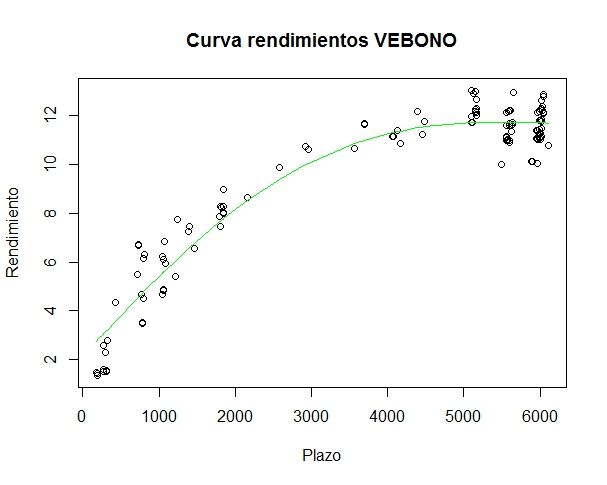
\includegraphics{images/curvarend.jpeg}}
\caption{Curva de rendimiento.}
\label{c_rend}
\end{figure}

\hspace{0.4cm} Como se dijo anteriormente, los resultados de los precios obtenidos mediante el uso de la metodolog\'ia de splines de suavizado ser\'an comparados con los precios obtenidos a trav\'es de la metodolog\'ia de Svensson. En dicha metodolog\'ia existe un proceso de optimizaci\'on el cual permite encontrar los par\'ametros id\'oneos, de tal manera que la diferencia entre los precios promedio de cada instrumento y su precio te\'orico sea lo m\'as peque\~na posible. El proceso de esta optimizaci\'on se muestra a continuaci\'on.


%\section{Elecci\'on \'optima del par\'ametro de suavizamiento.}

\newpage

\section{Proceso de optimizaci\'on de Svensson.}


\hspace{0.4cm} Para aplicar este proceso es necesario tener una funci\'on objetivo, sobre la cual se realizar\'a el proceso de optimizaci\'on, ya sea para maximizar \'o minimizar dicha funci\'on. Dependiendo de la forma de dicha funci\'on el proceso de optimizaci\'on ser\'a lineal o no lineal. En nuestro caso particular se llevar\'a a cabo un proceso de optimizaci\'on no lineal donde se buscar\'a minimizar la funci\'on objetivo.


\hspace{0.4cm} En el c\'alculo de nuestra funci\'on objetivo inteviene el concepto de la duraci\'on de un bono \'o t\'itulo, la cu\'al es una medida del vencimiento medio ponderado de todos los flujos que paga un bono. La misma viene dada mediante la siguiente expresi\'on, \\

\begin{center}

$\displaystyle{Duracion = \frac{1+r}{r} - \frac{n(c-r)+(1+r)}{c(1+r)^{n}-(c-r)}}$

\end{center}


\noindent donde

\begin{itemize}
  \item r es el rendimiento al vencimiento del bono durante el per\'iodo considerado.
  \item n es el n\'umero de per\'iodos que restan hasta la fecha de vencimiento del bono.
  \item c es el cup\'on del bono.
\end{itemize}


\hspace{0.4cm} As\'i nuestra funci\'on objetivo viene dada mediante la siguiente expresi\'on,

\vspace{0.2cm}

\begin{equation}\label{ecua2}
  f(x) = \sum_{i=1}^{n} (w_{i}\epsilon(x)_{i} )^2
\end{equation}


\noindent donde $w_{i}$ representan las ponderaciones, y se calculan mediante la siguiente expresi\'on,

\vspace{0.2cm}


\begin{center}

$\displaystyle{w_{i} = \frac{\frac{1}{D_{i}}}{\sum_{j=1}^{N}\frac{1}{D_{j}}}}$

\end{center}


\vspace{0.2cm}


\noindent por su parte, $\epsilon_{i}(x)= \hat{Pr}_{i}(x)-Pr_{i}$, donde $Pr_{i}$ representan los precios promedios de los t\'itulos a considerar, de entrada este es un par\'ametro \'o valor con el que se cuenta. Por otra parte $\hat{Pr}_{i}(x)$ representa los precios estimados donde $x$ es el par\'ametro que va a variar y es el valor que se quiere optimizar.


\hspace{0.4cm} Mediante la funci\'on objetivo descrita anteriormente se busca minimizar la diferencia que existe entre los precios promedios y los precios estimados, calculando un valor \'optimo del par\'ametro $x$ mediante el proceso de optimizaci\'on no lineal.



\hspace{0.4cm}El proceso de optimizaci\'on se realiz\'o mediante el software estad\'istico R, mediante el paquete ``nloptr". En este paquete, se encuentra el comando ``aulag" el cual minimiza un funci\'on objetivo y devuelve entre otros valores el par\'ametro m\'as \'optimo, que hace que la funci\'on sea m\'inima. Un ejemplo del uso de este comando se presenta acontinuaci\'on,

\begin{center}
  $ala2=auglag(1.22, fn=mifuncion, hin=res)$
\end{center}


\noindent donde el primer argumento debe ser el valor inicial del par\'ametro a optimizar, el segundo argumento ``fn" se refiere a la funci\'on que se desea optimizar, finalmente en el tercer par\'ametro ``hin" se indican las restricciones sobre el par\'ametro a optimizar, en este caso la restricci\'on establecida es que el par\'ametro sea mayor a cero.


\hspace{0.4cm} Recordemos que la tasa cero cup\'on que se obtiene mediante la metodolog\'ia de Svensson est\'a dada por la siguiente expresi\'on,\\


$\displaystyle{s(m) = \beta_{0}+ \beta_{1}\frac{\left(1-e^\frac{-m}{\tau_{1}}\right)}{m/\tau_{1}} + \beta_{2} \left(\frac{\left(1-e^\frac{-m}{\tau_{1}}\right)}{m/\tau_{1}} -  e^\frac{-m}{\tau_{1}}\right) + \beta_{3} \left(\frac{\left(1-e^\frac{-m}{\tau_{2}}\right)}{m/\tau_{2}} -  e^\frac{-m}{\tau_{2}}\right)}$\\

\noindent esta expresi\'on est\'a sujeta a las siguientes restricciones,

\begin{itemize}
  \item $\beta_{0} > 0$
  \item $\beta_{0}+\beta_{1} > 0$
  \item $\tau_{1} > 0$
  \item $\tau_{2} > 0$
\end{itemize}

\noindent cada par\'ametro controla una secci\'on de la curva. La f\'ormula anterior es de suma importancia ya que ella interviene en el c\'alculo del precio te\'orico de cada instrumento. El proceso de optimizaci\'on act\'ua directamente sobre esta f\'ormula, ya que el mismo se centra en variar los par\'ametros de tal manera que la funci\'on objetivo sea minimizada.

\hspace{0.4cm} Como se observ\'o en las secciones anteriores el par\'ametro de suavizamiento fu\'e elegido mediante el m\'etodo de ensayo y error el cual no es para nada \'optimo pues a priori este m\'etodo no nos garantiza que el valor seleccionado sea el mejor, ya que se contar\'ian con una gran cantidad de posibles valores a seleccionar, con el fin  de encontrar dicho par\'ametro el procedimiento anteriormente explicado puede ser implementado. 

\hspace{0.4cm} Sin embargo, al realizar este proceso, se obtienen curvas que no son para nada suaves y en ocasiones no poseen ningunas de las formas usuales de la curva de rendimientos. Esto es debido a que en este caso este proceso, var\'ia el par\'ametro de suavizamiento de tal manera que la diferencia entre el precio promedio y el precio te\'orico sea lo mas peque\~na posible y en este proceso no existe un par\'ametro que controle la forma de la curva obtenida. Por lo tanto, su aplicaci\'on presenta algunos inconvenientes.  





